Die vorgestellte erweiterte Form des Modells erleichtert Implementation und Verifikation. Große Teile des Modells sind statisch (vgl. \ref{eq:block_matrix_form}) und können im Voraus berechnet werden. Es sind nun auch die gemessenen Phasenwerte Teil des Modells, genauer: der Matrix $\mathbf{A}$. Im Folgenden werden die Auswirkungen auf die Kondition der Matrix betrachtet. Dazu wird Untersucht inwieweit die Zerlegung in Blockmatrizen und die Untersuchung der Kondition dieser eine Abschätzung der vollständigen Konditionszahl im Allgemeinen darstellt. 
%
\begin{equation}
\label{eq:block_matrix_form}
\mathbf{A}=\bigg( \mathbf{Z}\quad \mathbf{P}\quad \mathbf{V}\bigg)
\end{equation}
%
Dabei ist:
\begin{equation}
\mathbf{Z} \in \mathbb{R}^{3x3} \quad \mathbf{P} \in \mathbb{R}^{3x3} \quad \mathbf{V}\in \mathbb{R}^{4x3}
\end{equation}
%
Die Matrizen $\mathbf{Z}$ und $\mathbf{P}$ sind statisch. Hingegen enthält die Matrix $\mathbf{V}$ die gemessenen Phasenwerte $\Theta_k$ der Antennen für diese Konfiguration. \\
%
Die Abbildung~\ref{fig:CondNumberAnalyze} zeigt die bereits angestellte Untersuchung zu dieser Überlegung. Abbildung~\ref{fig:AnalyzeOf3x3} stellt die Konditionszahl der rein geometrischen $3\times3$-Matrix dar. In der Abbildung~\ref{fig:AnalyzeOf10x3} sehen wir die Kondition der erweiterten Matrix. Neben der geometrischen sind auch die beiden anderen Blockmatrizen in diese Konditionsbetrachtung eingeflossen. Als zusätzliche Angabe wird ist sind die Skalierungsfaktoren angegeben. Legt man beide Grafiken übereinander erkennt man:
\begin{enumerate}
\item Geometrisch gut konditionierte Konfigurationen (linke Grafik), bleiben im erweiterten Modell (rechte Grafik) weiterhin gut konditioniert.
\item Die Konditionszahl der \textit{schlechteste} ist wesentlich kleiner (ca. Faktor $10$) als im rein geometrischen Modell
\end{enumerate}
%
\begin{figure}[h]
         \centering
	     \caption[Ergebnisse der Konditionsanalyse alle Permutationen]{Analyse der Konditionszahlen aller möglichen Matrizen für den Messaufbau; Die Konditionszahl ist für jede mögliche Permutation an Messantennen für eine Referenzantenne angegeben}\label{fig:CondNumberAnalyze}
         \begin{subfigure}[h]{0.45\textwidth}
                 \centering
                 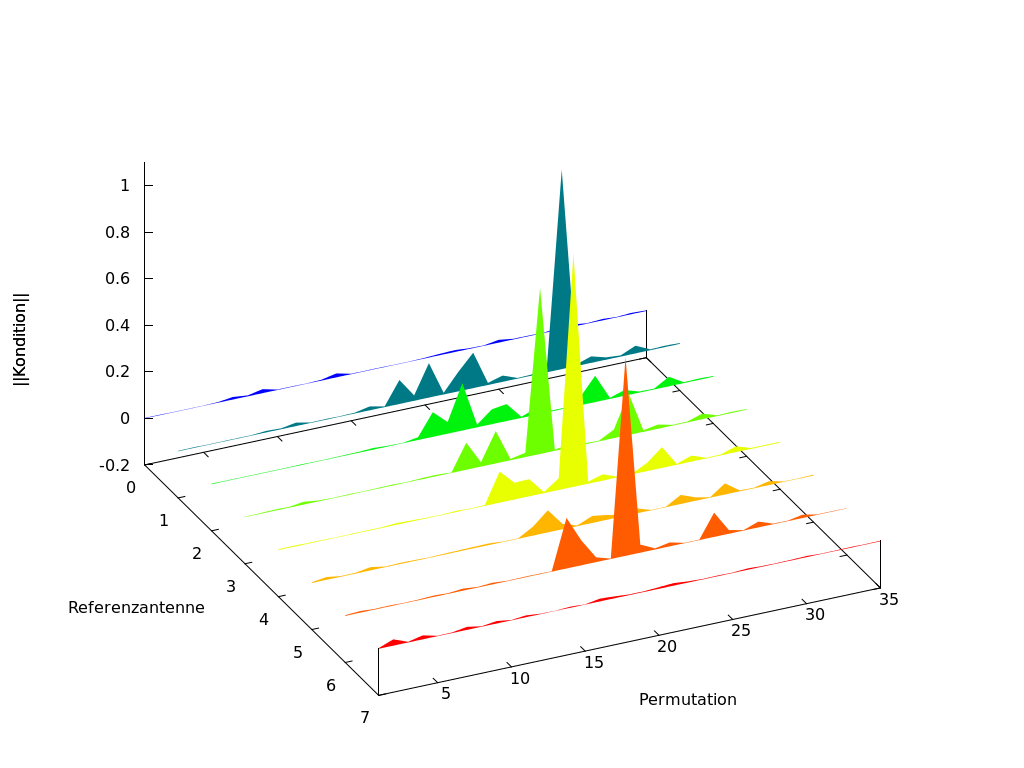
\includegraphics[width=\textwidth]{img/fenceModell3x3.png}
                 \caption{Konditionszahl der rein geometrischen $3\times3$ Matrix normiert auf den größten vorkommenden Wert ($=2149,16$). Auf den Achsen finden sich der Index der Referenzantenne sowie die Nummer der Permutation. Die z-Achse enthält die normierte Kondition}
                 \label{fig:AnalyzeOf3x3}
         \end{subfigure}
%         
         \begin{subfigure}[h]{0.45\textwidth}
                 \centering
                 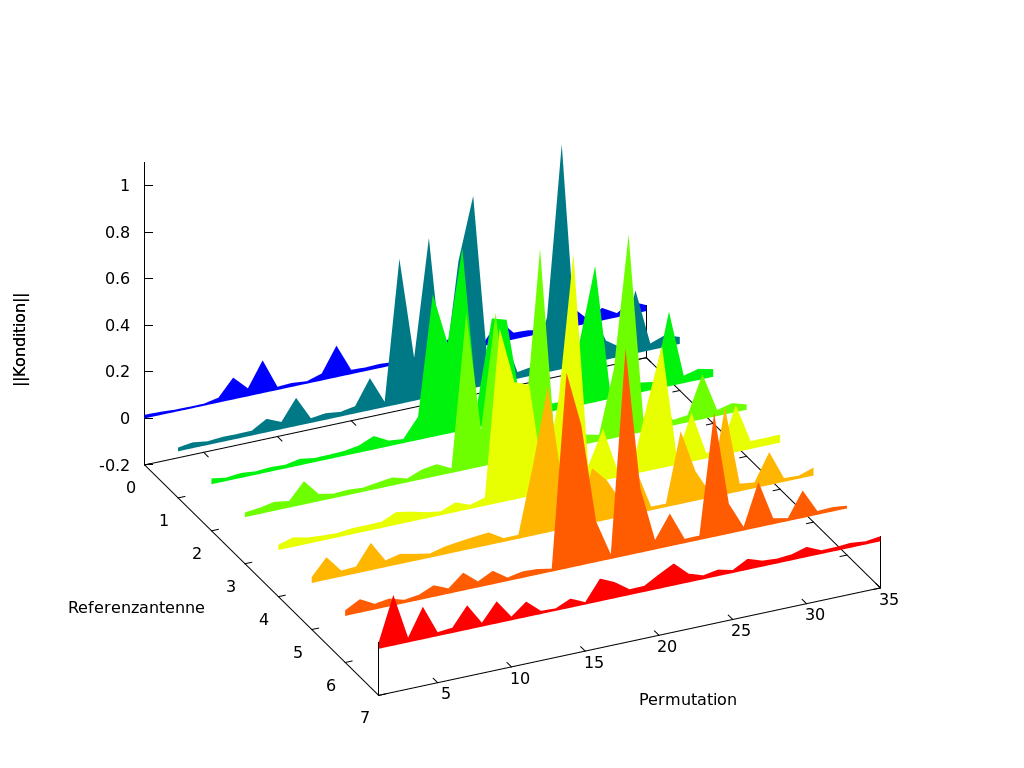
\includegraphics[width=\textwidth]{img/fenceModell9x3.png}
                 \caption{Konditionszahl der $10\times3$ Matrix normiert auf den größten vorkommenden Wert ($=257,13$); In dieser Konfiguration sind die Konstanten ($a_1$ \& $a_2$) sowie die variablen, gemessenen Phasen $\Theta_k$ enthalten}
                 \label{fig:AnalyzeOf10x3}
         \end{subfigure}
%
\end{figure}
%
Aus der Grafik lässt sich entnehmen, dass es für jede Referenzantenne aus der Geometrie alleine gute Konfigurationen existieren. Aus diesen Erkenntnissen kann in späteren Aufbauten, die Position der Antennen optimiert werden. Diese Verfahren wird in Abschnitt~\ref{sec:Calibration_Optimaztion} weiter beschrieben.
%
%- Section 2.3 --------------------------------------------------------------
\subsection{Weitere Anwendung der Konditionszahl}
Weitere Anwendungen, die sich aus der Konditionszahl der Matrix ableiten, sind denkbar. Für die FPGA-Software ist, parallel zu diesem Projekt, eine intelligente Umschaltung der Antennen in der Planung. Die Kondition der geometrische Matrix verändert sich nach dem Kalibrieren nicht mehr. Dadurch und durch die oben beschriebenen Überlegungen kann statisch eine Abschätzung für die Konditionszahl, von zwei der drei Blockmatrizen, im Vorfeld erstellt werden. Die Konditionszahl dient zum Steuern der Umschaltung. Ordner man die möglichen Konfiguration anhand ihrer Konditionszahl (niedrigste zuerst) in einer statischen Liste an so kann im FPGA eine einfache, schlaue Umschaltung implementiert werden. Diese würde immer dafür sorgen, dass Messdaten von einer Konfiguration bevorzugt werden, die eine niedrige Konditionszahl hat und somit relativ sicher zu einer guten Lösung führen. Diese überlegungen werden im Rahmen dieser Arbeit nicht näher beschrieben.\\
Eine Weitere Anwendung ergibt sich für die Kalibrierung. Der Aufbau der Antennen kann unter Berücksichtigung der Kondition optimieren. Ziel der Optimierung wäre es durch eine geeignete Positionierung der Antennen, die Anzahl der Antennenpermutationen mit kleiner Konditionszahl zu maximieren.